%=======================================================================
%  MATHEMATICAL METHODS IN COMPUTER SCIENCE, LECTURE NOTES
%=======================================================================
\def\lectureNr{1}   %enter number!
\def\lecture{Introduction to Optimization Problems and Mathematical Programming} %select and enter title
\def\scribe{Victor Glazer}           %enter your name


%%%%%%%%%%%%%%%%%%%%%%%%%%%%%%%%%%%%%%%%%%%%
% DON'T CHANGE ANYTHING IN THE NEXT LINES
\def\solitude{1} %KEEP THIS WAY!!!
\ifnum\solitude=1
 \documentclass[10pt]{article}
 % 'usegraphics' changed to 'nousegraphics' by VG
 \usepackage[nousetoc,nohylinks,nousegraphics]{lnotes}
\fi
%%%%%%%%%%%%%%%%%%%%%%%%%%%%%%%%%%%%%%%%%%%%

%Check if we are compiling under latex or pdflatex (added by VG)
\ifx\pdfoutput\undefined
  \usepackage[dvips]{graphicx}
\else
  \usepackage[pdftex]{graphicx}
\fi

%%%%%%%%%%%%%%%%%%%%%%%%%%%%%%%%%%%%%%%%%%%%%%%%%%%%%%%%%%%%%%%%
% YOU MAY ADD ADDITIONAL (PRIVATE) MACROS HERE,
% BUT DO START EACH WITH YOUR INITIALS.
% FOR EXAMPLE, YOUR NAMES IS ARIK SHARON
% THEN START EACH MACRO WITH AS.
% EXAMPLE:
%\newcommand{\ASnorm}[2]{\|#1\|_{_#2}}
\usepackage{enumerate,psfrag}
\newcommand{\VGnorm}[1]{||#1||}
\newcommand{\VGdom}{\mathcal{D}}
\newcommand{\VGfancyc}{\mathcal{C}}
\newcommand{\VGfancyf}{\mathcal{F}}
\newcommand{\VGfancyh}{\mathcal{H}}
\newcommand{\VGfancyt}{\mathcal{T}}
\newcommand{\VGzone}{[0,1]}
\newcommand{\VGrplus}{\R^{\geq 0}}
\newcommand{\VGxvec}{\vec{x}}
\newcommand{\VGyvec}{\vec{y}}
\newcommand{\VGzvec}{\vec{z}}
\newcommand{\VGbvec}{\vec{b}}
\newcommand{\VGcvec}{\vec{c}}
\newcommand{\VGorg}{\vec{0}}
\newcommand{\VGepi}{epi}
\newcommand{\VGhull}{hull}
\renewcommand{\qedsymbol}{$\blacksquare$}
%%%%%%%%%%%%%%%%%%%%%%%%%%%%%%%%%%%%%%%%%%%%%%%%%%%%%%%%%%%%%%%%

\BEGINDOC
\makeheader

% Set section counter to the current lecture number
% ADDED BY VG
\setcounter{section}{\lectureNr}
%%%%%%%%%%%%%%%%%%%%%%%%%%%%%%%%%%%%%%%%%%%%%%%%%%%%%%%%%%%%%%%%%%%%%%%%%
% BEGIN BODY of Document
\begin{summary}
Introduction to optimization problems in general and Mathematical Programming
in particular. Convex sets and functions. Convex and Linear Programming.
\end{summary}

\section*{Optimization Problems}

\begin{definition}
An \emph{optimization problem} consists of a set $\VGdom$, called the \emph{domain}, 
and a real-valued function $f: \VGdom \to \R$, called the \emph{objective
function}. $f(x) \in \R$ represents the ``profit'' or
``cost'' associated with $x \in \VGdom$.
\end{definition} 
%\begin{remark}
%It is often convenient to slightly abuse the above definition
%and allow objective functions of the form $f: \VGdom' \to \R$ for some
%$\VGdom' \supset \VGdom$.
%\end{remark}

\noindent
Optimization problems come in two flavours: minimization problems and maximization problems. 
In a {\it maximization problem}, the goal is to find an $x \in \VGdom$ such that $f(y) \leq f(x)$ for
all $y \in \VGdom$. In other words, we want a domain element which yields the
greatest profit. In a {\it minimization problem}, on the other hand, the goal
is to find an $x \in \VGdom$ such that $f(x) \leq f(y)$ for all $y \in \VGdom$.
In this case we want a domain element which has the smallest cost.

In general, $f$ may fail to have an optimum in $\VGdom$.
However, if $\VGdom$ is finite then every $f$ has both a
minimum and a maximum in $\VGdom$.

\bigskip\noindent
Let's look at a few examples.
\begin{enumerate}
\item
Let $p$ be a univariate polynomial. Where does $p$ attain its maximum value, if we restrict
it to the closed interval $\VGzone \subset \R$?

This is a maximization problem. The domain is $\VGdom = \VGzone$ and the objective
function $f$ is simply $p$ itself.

\item
\label{VG:exm:curves}
What is the largest area enclosed by a two-dimensional (closed) curve of
length one? 

This is a maximization problem. The domain $\VGdom$ consists
of all closed two-dimensional curves of unit length, and the objective function $f$ maps
a two-dimensional curve to the area enclosed by it.

\item
Recall the classical Minimum Spanning Tree (MST) problem. 
Suppose that we are given an undirected graph $G = (V,E)$ and a weight
function $w: E \to \R$. The weight $W$ of a subgraph $G'$ of $G$ with edge set
$E' \subseteq E$ is just the sum of the individual weights of its edges, 
$W(G') \eqdef \sum_{e \in E'}w(e)$. A {\it path} in $G$ is a sequence of 
vertices $v_1,\ldots,v_n \in V$, $n \leq |V|$ such that $(v_i,v_{i+1}) \in E$ for $1 \leq
i \leq n-1$. A {\it cycle} is a closed path, so that $v_1 = v_n$. $G$ is 
{\it connected} if there is a path between every $u,v \in V, u \neq v$, and {\it acyclic} if it
doesn't contain any cycles. A {\it spanning tree} $T$ of $G$ is a 
connected acyclic subgraph of $G$ with vertex set $V$. What is the least-weight 
spanning tree of $G$? 

This is a minimization problem. The domain is $\VGfancyt(G) \eqdef \{T : T
\text{ is a spanning}\\ \text{tree of } G\}$, and the objective function is the
sum of the edge weights, $W$. Notice that here the domain is finite,
unlike in the previous two examples, since $|\VGfancyt(G)| \leq 2^{|E|}$. This problem is {\it
tractable}, meaning that there are polynomial-time algorithms for it
(where by {\it polynomial time} we mean {\it deterministic} polynomial time
{\it in the worst case}). The two best-known ones are due to Prim
\cite{Prim57} and Kruskal \cite{Kruskal56}, whereas Chazelle's \cite{Chazelle00} is 
currently the fastest.

\item Another classical optimization problem is the
Travelling Salesman Problem (TSP). We are given an undirected graph $G =
(V,E)$, whose vertices represent cities, and a pairwise distance function $d:
E \to \R$; $d(u,v)$ is the distance between cities $u, v \in V$. A {\it
Hamiltonian cycle} in $G$ is a cycle in which every $v \in V$ appears exactly
once. The {\it length} $L$ of a cycle $C = v_1,\ldots,v_n$ is the sum of the distances
between adjacent vertices, $L(C) \eqdef \sum_{i = 1}^{n-1} d(v_i,v_{i+1}) + d(v_n,v_1)$.  
What is the shortest Hamiltonian cycle in $G$?

This is a minimization problem. The domain is $\VGfancyh(G) \eqdef \{H : H
\text{ is a}\\ \text{Hamiltonian cycle in } G\}$ and the objective function is the cycle length
$L$. As with the MST problem, the domain here is finite. Unlike the MST problem, however, TSP is {\it
intractable}, since it is NP-hard (and therefore does not have a
polynomial-time algorithm unless $P = NP$). 

\item
\label{VG:exm:flows}
A {\it flow network} is a directed graph $G = (V,E)$ together with a 
{\it capacity function} $c: E \to \VGrplus$ and two distinguished vertices $s,t
\in V$; $s$ is called the {\it source} and $t$ is called the {\it sink}. For
every $v \in V$, let $IN(v) \eqdef \{e \in E : e = (u,v) \text{ for some } u \in
V\}$ and $OUT(v) \eqdef \{e \in E : e = (v,u) \text{ for some } u \in V\}$. 
\begin{minipage}{\textwidth}
A {\it flow} in $G$ is a function $f: E \to \R$ which satisfies the
following three conditions: 
\begin{enumerate}[(i)]
\item Non-negativity: for all $e \in E$, $f(e) \geq 0$
\item Capacity Constraints: for all $e \in E$, $f(e) \leq c(e)$ 
\item Flow conservation: for all $v \in V$, $\sum_{e \in IN(v)} f(e) = 
\sum_{e \in OUT(v)} f(e)$
\end{enumerate}
\end{minipage}

Intuitively, the capacity constraints ensure that the flow along a given edge
does not exceed that edge's capacity, and the matter conservation constraints
ensure that the flow entering a given vertex is equal to the flow exiting it.
The {\it size} of a flow $f$ is $\VGnorm{f} \eqdef \sum_{e \in OUT(s)}f(e) -
\sum_{e \in IN(s)}f(e)$. What is the largest flow in $G$?

This is a maximization problem. The domain is $\VGfancyf(G) \eqdef \{f : f \text{ is a
flow in } G\}$ and the objective function is the flow size $||\! \cdot \! ||$.
Although $\VGfancyf(G)$ is infinite, the problem is 
tractable. One of the best-known algorithms --- though not the most efficient
--- is due to Edmonds and Karp \cite{EdmondsKa72}; it fits into Ford and Fulkerson's {\it augmenting
paths} framework \cite{FordFu62}. The fastest algorithms currently known are of the 
push-relabel variety \cite{GoldbergTa88}.

An interesting aspect of network flows is
the {\it Max flow/Min cut} theorem. A {\it cut} in $G$ is a partition of the
vertex set $V$ into disjoint sets $S$ and $T$ such that $S \cup T = V$, $s \in
S$ and $t \in T$. The {\it capacity} $C$ of a cut $(S,T)$ is $C(S,T) \eqdef \sum_{e \in E(S,T)} c(e)$, 
where $E(S,T) \eqdef \{(u,v) \in E : u \in S, v \in T\}$. Denote the set of
all cuts in $G$ by $\VGfancyc(G) \eqdef \{(S,T): (S,T) \text{ is a cut in }
G\}$. We call $f$ a {\it maximum flow} in $G$ if it has the largest size possible, so that $\VGnorm{f} =
\max\{\VGnorm{f'} : f' \in \VGfancyf (G) \}$, and $(S,T)$ a {\it minimum cut} in $G$ 
if it has the smallest size possible, so that $C(S,T) = \min\{C(S',T') : (S',T') \in
\VGfancyc(G)\}$.

\begin{theorem} 
The size of the maximum flow in $G$ is equal to the capacity of the minimum cut in $G$.
\end{theorem}

This is a special case of {\it Linear Programming \emph{(LP)} duality}, a concept
we will explore in greater detail later in the course.
\end{enumerate}

\section*{Mathematical Programming}
Although the above setting is very general, it is too abstract to
be algorithmically interesting. We next consider {\it mathematical
programming}, a more concrete special case. 

\begin{definition}
A \emph{mathematical program} consists of an objective function $f: \R^n \to
\R$, a set of $m$ \emph{constraint functions} $\{g_i : \R^n \to \R\}_{i =
1}^{m}$ and a \emph{constant vector} $\VGbvec = (b_1,\ldots,b_m) \in \R^m$.
The goal is to find an $\VGxvec \in \VGdom$ which minimizes $f(\VGxvec)$, where
the domain $\VGdom \subseteq \R^n$ is defined implicitly by the inequality constraints
$g_i(\VGxvec) \leq b_i, 1 \leq i \leq m$, $\VGdom = \bigcap_{i = 1}^m \{ \VGxvec \in \R^n : g_i(\VGxvec)
\leq b_i \} = \{ \VGxvec \in \R^n : g_i(\VGxvec) \leq b_i, 1 \leq i \leq m \}$.
\end{definition}

\noindent
We usually write such programs as follows:
\begin{align*}
& \min f(\VGxvec) \quad  \text{subject to}\\ 
& g_i(\VGxvec) \leq b_i \quad \text{for } i = 1 \ldots m
\end{align*}

\noindent
Since the domain is restricted to be some subset of $n$-dimensional
Euclidean space, this a more limited setting. Some problems, like
example \ref{VG:exm:curves} above for instance, cannot be cast as mathematical programs. 
Mathematical programming is still too general for our purposes, however, since
it allows for intractable problems. 
We prefer to concentrate on certain special cases involving ``nice'' 
$f$'s and $g$'s, for various notions of ``niceness''.

\subsection*{Convex Programming}
First, we'll need some definitions.

\begin{definition}
A set $S \subseteq \R^n$ is {\it convex} if $\lambda \VGxvec + (1 -
\lambda)\VGyvec \in S$ for all $\VGxvec,\VGyvec \in S$ and $\lambda \in \VGzone$.
\end{definition}

\noindent
Geometrically, $S$ is convex if every line segment joining two points
in $S$ is contained in $S$. 

We can view the point $\lambda \VGxvec + (1 - \lambda)\VGxvec$
as a ``weighted average'' of $\VGxvec$ and $\VGyvec$, the weights being $\lambda$
and $(1 - \lambda)$, which are non-negative and sum to 1. 
Such averages are called {\it convex combinations}. If $S$ is 
convex then every convex combination of points in $S$ also lies
in $S$, so that $S$ is ``closed under taking convex combinations''. 

\bigskip\noindent
{\bf Examples of convex sets:} $\varnothing$, the unit $n$-ball 
$\{\VGxvec \in \R^n : \normtwo{\VGxvec} \leq 1\}$, any affine subspace of $\R^n$, 
the first set depicted in \figureref{VG:fig:sets}.

\medskip\noindent
{\bf Examples of non-convex sets:} $\R^n \setminus \{\VGorg\}$, the second
set depicted in \figureref{VG:fig:sets}.

\bigskip
\begin{figure}[h]
    \centering
    
\includegraphics[width = 0.2\textwidth]{convex_set}
    \hspace{0.1\textwidth}
    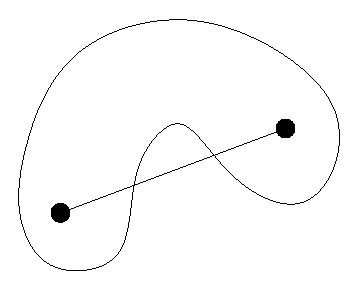
\includegraphics[width = 0.2\textwidth]{nonconvex_set}
    \caption{A convex set (left) and one that isn't (right).}
    \label{VG:fig:sets}
\end{figure}

\begin{definition}
Let $S \subseteq \R^n$ be a convex set. 
A function $f:S \to \R$ is \emph{convex} 
if $f(\lambda \VGxvec + (1 - \lambda)\VGyvec) \leq \lambda f(\VGxvec) + (1 -
\lambda) f(\VGyvec)$ for every $\VGxvec,\VGyvec \in S$ and $\lambda \in \VGzone$.
Notice that $\VGzvec = \lambda \VGxvec + (1 - \lambda)\VGyvec \in S$ by convexity of $S$, 
so it makes sense to evaluate $f$ on $\VGzvec$. 
\end{definition}

\noindent
In other words, $f$ is a convex function if the image under $f$ of every convex 
combination of points in $S$ is bounded above by the convex combination of their images.

Geometrically, $f$ is convex if its {\it epigraph}, $\VGepi(f)
\eqdef \{(\VGxvec,y) \in \R^{n+1} : \VGxvec \in S, y \geq
f(\VGxvec)\}$, is a convex set. For univariate functions, this means that the line
segment joining any two points on the graph of $f$ lies on or above the graph.

\begin{figure}
    \centering
    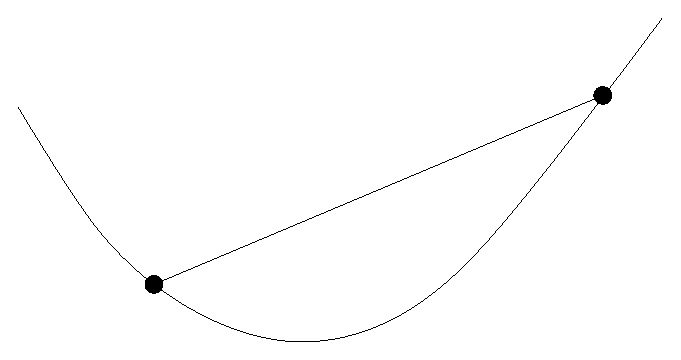
\includegraphics[width = 0.5\textwidth]{convex_fun}
    \caption{A convex function.}
    \label{VG:fig:conv_fn}
\end{figure}

\bigskip\noindent
{\bf Examples of convex functions:} linear functions (see below), norms
(ditto), $x^k$ for $x \in \VGrplus$ and $k \in \N$, the function
depicted in \figureref{VG:fig:conv_fn}.

\medskip\noindent
{\bf Examples of functions which \emph{aren't} convex:} $f(x) = \sqrt{x}, x
\in \VGrplus$.

\bigskip\noindent
To verify that $\sqrt{x}$ is \emph{not} convex, note that 
\[
\sqrt{\frac{1}{2}0
+ \frac{1}{2}100} = \sqrt{50} \approx 7.07 > 5 = \frac{1}{2}\sqrt{0} +
\frac{1}{2}\sqrt{100}. 
\]
Recall that a {\it norm} is any function $||\! \cdot \!||: \R^n \to \R$ which
satisfies the following three conditions:

\begin{enumerate}[(i)]
\item $\VGnorm{\VGxvec} > 0$ for all $\VGxvec \in \R^n \setminus \{\VGorg\}$,
and $f(\VGorg) = 0$
\item $\VGnorm{c\VGxvec} = |c|\ \VGnorm{\VGxvec}$ for all $\VGxvec \in \R^n$ and $c \in \R$
\item $\VGnorm{\VGxvec + \VGyvec} \leq \VGnorm{\VGxvec} + \VGnorm{\VGyvec}$ for all
$\VGxvec,\VGyvec \in \R^n$ (triangle inequality)
\end{enumerate}

\begin{claim}
\label{VG:clm:norms_convex}
Norms are convex functions.
\end{claim}

\begin{proof}
Let $f: \R^n \to \R$ be a norm, $\VGxvec,\VGyvec \in \R^n$ 
and $\lambda \in \VGzone \subseteq \R$. We have:

\begin{align*}
\VGnorm{\lambda \VGxvec + (1-\lambda) \VGyvec} & \leq \VGnorm{\lambda
\VGxvec} + \VGnorm{(1 - \lambda)\VGyvec}
\quad (\text{by the triangle inequality)}\\
& = |\lambda| \ \VGnorm{\VGxvec} + |(1 - \lambda)| \ \VGnorm{\VGyvec} \quad \text{(by property
(ii) of norms)}\\
& = \lambda \VGnorm{\VGxvec} + (1 - \lambda) \VGnorm{\VGyvec} \quad \text{ (since }
\lambda, 1-\lambda \geq 0).
\end{align*}

\end{proof}

\noindent
We are now ready to define Convex Programming.

\begin{definition}
A mathematical program 
\begin{align*}
& \min f(\VGxvec) \quad \text{subject to}\\ 
& g_i(\VGxvec) \leq b_i \quad \text{for } i = 1 \ldots m
\end{align*}
is {\it convex} if both the objective function $f: \R^n \to \R$ and the constraint functions 
$g_i: \R^n \to \R, 1 \leq i \leq m$ are convex.
\end{definition}

\noindent
Here the domain is a convex set, as we will show in a moment. 
We'll need the following two lemmas.

\begin{lemma}
\label{VG:lem:int_conv}
The intersection $S = \bigcap_{i=1}^m S_i$ of a collection of $m$ convex sets
$\{S_i\}_{i=1}^m$ is itself convex. 
\end{lemma}
\begin{proof}
Let $\VGxvec,\VGyvec \in S = \bigcap_{i=1}^m S_i$ and $\lambda \in \VGzone$. Since 
$\VGzvec = \lambda \VGxvec + (1-\lambda)\VGyvec \in S_i$ for all $1 \leq i
\leq m$ (by convexity of the individual $S_i$'s), $\VGzvec \in \bigcap_{i=1}^m S_i = S$.
\end{proof}

\begin{lemma}
\label{VG:lem:dis_conv}
Let $g: \R^n \to \R$ be a convex function and $b \in \R$ be a constant. 
Then the set $S = \{\VGxvec \in \R^n : g(\VGxvec) \leq b \} \subseteq \R^n$ is convex.
\end{lemma}

\begin{proof}
Let $\VGxvec,\VGyvec \in S$ and $\lambda \in \VGzone$. We want to show
that $\lambda \VGxvec + (1-\lambda)\VGyvec \in S$, i.e. 
$g(\lambda \VGxvec + (1-\lambda) \VGyvec) \leq b$. We have:
\begin{align*}
g(\lambda \VGxvec + (1-\lambda) \VGyvec) & \leq \lambda g(\VGxvec) +
(1-\lambda) g(\VGyvec) \quad \text{ (by convexity of } g)\\
& \leq \max\{g(\VGxvec), g(\VGyvec)\} \quad \text{ (because } \lambda +
(1-\lambda) = 1)\\
& \leq b \quad \text{ (since } \VGxvec,\VGyvec \in S).
\end{align*}
\end{proof}

\noindent
The following theorem is an immediate consequence of lemmas
\ref{VG:lem:int_conv} and \ref{VG:lem:dis_conv}.
\begin{theorem}
\label{VG:thm:dom_conv}
The domain $\VGdom = \bigcap_{i = 1}^m \VGdom_i, \VGdom_i =\{ \VGxvec \in \R^n : g_i(\VGxvec)
\leq b_i \}$ of a convex program 
\begin{align*}
& \min f(\VGxvec) \quad \text{subject to}\\ 
& g_i(\VGxvec) \leq b_i \quad \text{for } i = 1\ldots m
\end{align*}
is a convex set.
\end{theorem}

\noindent
Let $\VGdom$ be a non-empty subset of $\R^n$ and $f: \R^n \to \R$ be a
function. Recall that $\VGxvec \in \VGdom$ is a {\it local
minimum} of $f$ in $\VGdom$ if $f(\VGxvec)$ is the smallest value
of $f$ in some $n$-ball contained in $\VGdom$ centered at $\VGxvec$. 
More formally, there exists an $\epsilon \in \R^{>0}$ such that $f(\VGxvec) \leq f(\VGyvec)$ for all
$\VGyvec \in \VGdom$ which satisfy $\normtwo{\VGxvec - \VGyvec} \leq \epsilon$
(where $|| \! \cdot \! ||_2$ denotes the Euclidean norm, see
\exampleref{VG:exm:norms}). If $f(\VGxvec) \leq f(\VGyvec)$ for all $\VGyvec \in
\VGdom$, then $\VGxvec$ is a {\it global minimum} of $f$ in $\VGdom$. Local and global maxima are
defined similarly. 

One reason general optimization problems are so difficult is that there may be
many local optima, some far from a global optimum. This means that
locally optimal decisions do not necessarily result in a solution which is globally 
optimal, or even close to one. However, this is not an issue in Convex
Programming, as the next theorem demonstrates.  

\begin{theorem}
\label{VG:thm:global_min}
Let $f: \R^n \to \R$ be a convex function. Then every local minimum $\VGxvec
\in \VGdom$ of $f$ in a convex set $\VGdom \subseteq \R^n$ is a global minimum
of $f$ in $\VGdom$.
\end{theorem}

\begin{proof}
Let $\VGzvec \in \VGdom$ be an arbitrary point in the domain
and $\VGxvec \in \VGdom$ be a local minimum of $f$ in $\VGdom$ (so that
$f(\VGxvec) \leq f(\VGyvec)$ for all $\VGyvec \in \VGdom$ such that
$\VGnorm{\VGxvec - \VGyvec} \leq \epsilon$, where $\epsilon > 0$ is some real
constant). Consider any convex combination $\VGyvec = \lambda \VGxvec +
(1-\lambda)\VGzvec$, $\lambda \in \VGzone$ of $\VGxvec$ and $\VGzvec$ which
is ``close'' to $\VGxvec$, so that $\VGnorm{\VGxvec - \VGyvec} \leq \epsilon$.
Since $\VGyvec \in \VGdom$ by convexity of $\VGdom$ and $\VGxvec$ is a local
minimum of $f$, we have 
\begin{align*}
f(\VGxvec) \leq f(\VGyvec) &= f(\lambda \VGxvec + (1-\lambda)\VGzvec)\\
& \leq \lambda f(\VGxvec) + (1-\lambda) f(\VGzvec) \text{ (by convexity of } f)\\
\end{align*}
so that $(1 - \lambda)f(\VGxvec) \leq (1-\lambda)f(\VGzvec)$. Since
$1-\lambda \geq 0$, this shows that $f(\VGxvec) \leq f(\VGzvec)$.
\end{proof}

\noindent
See \figureref{VG:fig:global_min} for a picture of the proof. 

\begin{figure}[h]
    \centering
    \psfrag{x}{$x$}
    \psfrag{y}{$y$}
    \psfrag{z}{$z$}
    \psfrag{e}{$\epsilon$}
    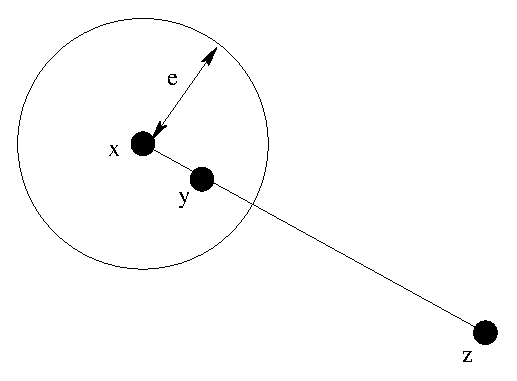
\includegraphics[width = 0.5\textwidth]{global_min}
    \caption{A graphical view of \theoremref{VG:thm:global_min}.}
    \label{VG:fig:global_min}
\end{figure}

\begin{example}
\label{VG:exm:norms}
Recall that the $\ell_2$ or {\it Euclidean} norm of $\VGxvec = (x_1,\ldots,x_n)
\in \R^n$ is $\normtwo{\VGxvec} \eqdef \sqrt{\sum_{j=1}^n x_j^2}$, whereas its
$\ell_1$ or {\it Manhattan} norm is $\normone{\VGxvec} \eqdef \sum_{j=1}^n |x_j|$.
What vector $\VGxvec = (x_1,x_2) \in \R^2$ in the first quadrant has the smallest
Euclidean norm, subject to the constraint that its Manhattan norm is 1? 
Since $\VGxvec$ lies in the first quadrant, so that $\sum_{j=1}^2|x_j| =
\sum_{j=1}^2 x_j$, we get the following program: 
\begin{align*}
\min \sqrt{x_1^2 + x_2^2} \quad \text{subje}&\text{ct to}\\
x_1 & \geq 0 \\
x_2 & \geq 0 \\
x_1 + x_2 & = 1
\end{align*}
However, this program doesn't quite have the right form, so we split the equality constraint 
and flip the $\geq$ constraints, obtaining
\begin{align*}
\min \sqrt{x_1^2 + x_2^2} \quad \text{sub}&\text{ject to}\\
-x_1 & \leq 0 \\ 
-x_2 & \leq 0 \\
x_1  + x_2 & \leq 1\\
-x_1 - x_2 & \leq -1
\end{align*}
The objective function is convex since it's a norm (see
Claim~\ref{VG:clm:norms_convex}), and the constraints are convex because they're linear (see
\definitionref{VG:def:linear}).
\end{example}

\subsection*{Linear Programming}
Linear Programming is an important special case of Convex Programming which
has been studied extensively over the past sixty years or so.

\begin{definition}
\label{VG:def:linear}
A function $f: \R^n \to \R$ is \emph{linear} if 

\begin{enumerate}[(i)]
\item $f(\VGxvec + \VGyvec) = f(\VGxvec) + f(\VGyvec) \quad \text{and}$
\item $f(\alpha \VGxvec) = \alpha f(\VGxvec)$
\end{enumerate} 

\noindent
for all $\VGxvec, \VGyvec \in \R^n$ and $\alpha \in \R$. 
\end{definition}

\noindent
\begin{observation}
\label{VG:rem:linear_fns}
Every linear function $f: \R^n \to \R$ can be expressed as
\[
f(\VGxvec) = \dprod{\VGcvec}{\VGxvec} = \sum_{j=1}^n c_j x_j,
\]
where $c_j = f(\vec{e}_j)$ and $\vec{e}_j$ is the $j^{th}$ {\it standard basis
vector} (which has a 1 in the $j^{th}$ coordinate and 0's everywhere else). 
\end{observation}

\begin{claim}
Linear functions are convex.
\end{claim}

\begin{proof}
Let $f: \R^n \to \R$ be a linear function, $\VGxvec,\VGyvec \in \R^n$ and
$\lambda \in \VGzone$. Then 

\begin{align*}
f(\lambda \VGxvec + (1-\lambda)\VGyvec) & = f(\lambda \VGxvec) + f((1 -
\lambda)\VGyvec) \quad \text{ (by linearity property (i))}\\
& = \lambda f(\VGxvec) + (1-\lambda)f(\VGyvec) \quad \text{ (by linearity
property (ii))}\\ 
& \leq  \lambda f(\VGxvec) + (1-\lambda)f(\VGyvec),
\end{align*}
\end{proof}

\noindent
In other words, for linear functions the image of a convex combination of two points
in the domain is actually equal to the convex combination of their images, as opposed to just being
upper-bounded by it.

\begin{definition}
A convex program 
\begin{align*}
& \min f(\VGxvec) \quad \text{subject to }\\ 
& g_i(\VGxvec) \leq b_i \quad \text{for } i = 1\ldots m
\end{align*}
is {\it linear} if both the objective function $f: \R^n \to \R$ and the constraint functions 
$g_i: \R^n \to \R, 1 \leq i \leq m$ are linear, and can therefore be expressed
as $f(\VGxvec) = \sum_{j=1}^n c_j x_j$, $g_i(\VGxvec) = \sum_{j=1}^n
a_{ij}x_j$ (see Observation~\ref{VG:rem:linear_fns}). The program then becomes
\begin{align*}
& \min \sum_{j=1}^n c_j x_j \quad \text{subject to}\\
& \sum_{j=1}^n a_{ij} x_j \leq b_i \quad \text{for } i = 1 \ldots m
\end{align*}
\end{definition}
\begin{example}
{\bf (the diet problem)} A farmer wants his cow to be as skinny as possible while still
keeping her healthy. There are $n$ different food types available, the $j^{th}$ food
containing $c_j \in \R$ calories per kilogram, $1 \leq j \leq n$, and $a_{ij} \in \R$ 
milligrams of vitamin $i$ per kilogram, $1 \leq i \leq m$. The cow requires at least $b_i \in \R$ 
milligrams of vitamin $i$ to stay healthy. Given that the goal is to minimize
caloric intake while having enough of each vitamin, how should she be fed? 

\medskip\noindent
Letting $x_j$ be the number of kilograms of food $j$ the cow is fed, 
we get the following linear program:
\begin{align*}
\min \sum_{j=1}^n & c_j x_j \quad \text{subject to} \\
x_j & \geq 0 \quad \text{for } j = 1 \ldots n\\
\sum_{j=1}^n a_{ij} x_j & \geq b_i \quad \text{for } i = 1 \ldots m
\end{align*}
\end{example}
\begin{example}
{(\bf network flows redux)} Recall the network flows problem from example \ref{VG:exm:flows}. 
As we already pointed out, fairly efficient specialized algorithms for this problem are
known. However, it can also be attacked using the general methods of Linear
Programming, as we now show.

\medskip\noindent
Letting $x_e$ be the flow along edge $e \in E$, $f(e)$, we get the following linear
program: 
\begin{align*}
\max \sum_{e \in OUT(s)} x_e & - \sum_{e \in IN(s)} x_e \quad \text{subject to} \\
x_e & \geq 0 \quad \text{for } e \in E \\ 
x_e & \leq c(e) \quad \text{for } e \in E \\
\sum_{e \in OUT(v)} x_e & = \sum_{e \in IN(v)} x_e \quad \text{for } v \in V \setminus \{s,t\} 
\end{align*}
\end{example}

% END BODY of document
%%%%%%%%%%%%%%%%%%%%%%%%%%%%%%%%%%%%%%%%%%%%%%%%%%%%%%%%%%%%%%%%%%%%%%%%%
\ENDDOC

%%%%%%%%%%%%%%%%%%%%%%%%%%%%%%%%%%%%%%%%%%%%%%%%%%%%%%%%%%%%%%%%%%%%%%%%%%%%%%%%%%%%%%%%%%%%%%%%%%%%%%%%%%%%%%%%%%%%%%%%%%%%%%%%


